\section{Auswertung}
\subsection{Die Drillachse}
\subsubsection{Die Winkelrichtgröße}\label{subsubsec:D}
Um die Winkelrichtgröße $D$ der Drillachse zu bestimmen wird Gleichung
\eqref{eq:D}
verwendet. Die Ergebnisse werden über die Formel für den Mittelwert
\[\bar{D}=\frac{1}{N}\sum_{i=1}^ND_.i\]
gemittelt und für die Bestimmung der Abweichung wird die Formel
\[\sigma_.D=\sqrt{\frac{1}{N(N-1)}\sum_{i=1}^N(D_.i-\bar{D})^2}\]
verwendet.\newline
Die benötigten Werte für die Kraft $F$, den Radius $r$ und den Winkel $\phi$, sowie die zugehörigen Werte für $D$ lassen sich der Tabelle \ref{tab:tab1}
entnehmen. Es ergibt sich für $\bar{D}$:
\[\bar{D}=\SI{2,56(6)e-2}{\joule}\]
\begin{table}
	\centering
	\caption{Messdaten zur Winkelrichtgrößenbestimmung.}
	\sisetup{table-format=1.2}
	\begin{tabular}{S[table-format=1.2] S[table-format=2.1]S[table-format=1.3]S[table-format=1.4]}
		\toprule
		{$F/\si[per-mode=reciprocal]{\newton}$}&{$r/\si[per-mode=reciprocal]{10^{-2}\metre}$}&{$\phi/\si[per-mode=reciprocal]{\radian}$}&{$D/\si[per-mode=reciprocal]{10^{-2}\joule}$} \\
		\midrule
		0,12 & 11,9 & 0,524 & 2,73 \\
		0,19 & 11,9 & 0,873 & 2,59 \\
		0,38 &  5,9 & 0,873 & 2,57 \\
		0,16 & 19,0 & 1,047 & 2,90 \\
		0,20 & 17,0 & 1,222 & 2,78 \\
		0,30 & 11,0 & 1,396 & 2,36 \\
		0,28 & 13,9 & 1,571 & 2,48 \\
		0,27 & 15,9 & 1,745 & 2,46 \\
		0,30 & 17,0 & 2,094 & 2,43 \\
		0,22 & 23,9 & 2,269 & 2,32 \\
		\bottomrule
	\end{tabular}
	\label{tab:tab1}
\end{table}
\subsubsection{Eigenträgheitsmoment}\label{subsubsec:I_D}
Zur Bestimmung des Eigenträgheitsmoments werden zwei Zylinder mit dem Durchmesser $d = \SI{3,5e-2}{\metre}$, der Höhe $h = \SI{3e-2}{\metre}$ und der Masse $m = \SI{221,8e-3}{\kilogram}$ verwendet.\newline
Die Verbindungsstange wird als masselos angenommen und wird daher nicht berücksichtigt.
Die Werte für das Quadrat der Periodendauer $T$ und des Abstandes $a$ aus Tabelle \ref{tab:tab2} sind im Graph \ref{fig:abb2} gegeneinander aufgetragen. Mittels der linearer Regression $T^2(a) = m \cdot a^2 + T_0^2$, ergeben sich mit Matplotlib \cite{matplotlib} für die Parameter $m$ und $T_0^2$:
\begin{align*}
m 	   &= \SI{751(6)}{\second\squared\per\metre\squared} \\
T_.0^2 &= \SI{5,1(2)}{\second\squared}
\end{align*}
%Dabei berechnen sich die Werte für $m$ und $n$ über:
%\begin{align*}
%m 	&= \frac{N\sum_{i=1}^N a_i^2 T_i^2 -\sum_{i=1}^N a_i^2 \sum_{i=1}^N T_i^2}{\Delta}\\
%n 	&= \frac{\sum_{i=1}^N a_i^4 \sum_{i=1}^N T_i^2 -\sum_{i=1}^N a_i^2 \sum_{i=1}^N a_i^2 T_i^2}{\Delta}
%\end{align*}
%und deren Abweichungen über:
%\begin{align*}
%\sigma_.m 	&= \sigma_.y\sqrt{\frac{N}{\Delta}}\\
%\sigma_.n 	&= \sigma_.y\sqrt{\frac{\sum_{i=1}^N a_i^4}{\Delta}},
%\end{align*}
%wobei $\Delta$ und $\sigma_.y$ definiert sind als:
%\begin{align*}
%\Delta 		&= N\sum_{i=1}^N a_i^4 -\left(\sum_{i=1}^N a_i^2\right)^2\\
%\sigma_.y 	&= \sqrt{\frac{1}{N-2}\sum_{i=1}^N \left(T_i^2-n-ma_i^2\right)^2}
%\end{align*}
Die Trägheitsmomente der Zylinder berechnen sich nach Formel \eqref{eq:I_SZH} zu:
\[I_.{ZH}=\SI{3,36e-5}{\kilogram\metre\squared}\]
Mit Gleichung \eqref{eq:I_D} ergibt sich für das Trägheitsmoment $I_.D$ der Drillachse:
\[I_.D=\SI{3,2(1)e-3}{\kilogram\metre\squared}\]
Die Messungenauigkeit ergibt sich dabei aus der Formel der Gaußschen Fehlerfortpflanzung
\begin{align*}
\sigma_.{I_.D}	&= \sqrt{\left(\frac{\partial (I_.D)}{\partial (T^2_.0)} \cdot \sigma_.{T^2_.0}\right)^2+\left(\frac{\partial (I_.D)}{\partial D}\cdot\sigma_.D\right)^2}\\
				&= \sqrt{\left(\frac{D}{4\pi^2}\cdot\sigma_.{T^2_.0}\right)^2+\left(\frac{T^2_.0}{4\pi^2}\cdot\sigma_.D\right)^2},
\end{align*}
wobei $\sigma_.{T^2_.0}$ der Fehler des Achsenabschnitts und $D$ und $\sigma_.D$ aus Abschnitt \ref{subsubsec:D} bekannt sind.
\begin{figure}
\centering
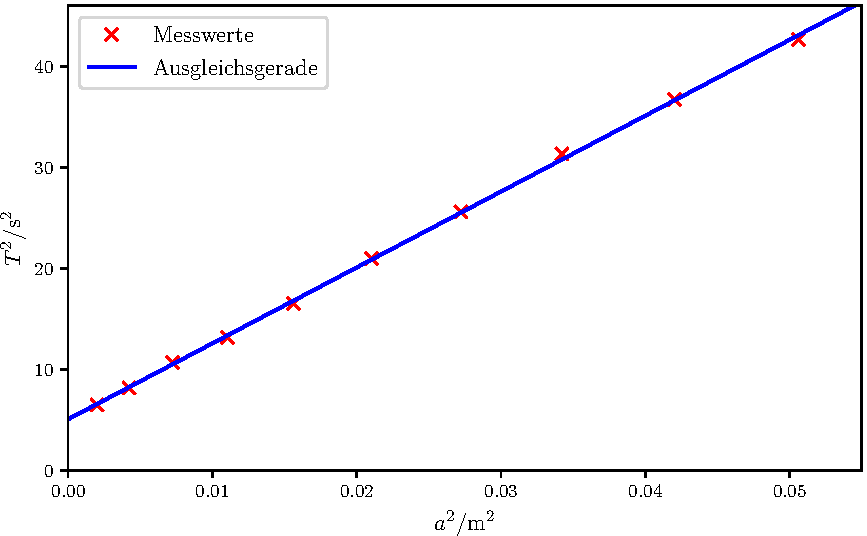
\includegraphics[scale = 0.75,keepaspectratio]
	{content/images/Graph.pdf}
\caption{Graph der Messdaten zur Bestimmung des Eigenträgheitsmoments der Drillachse mit Ausgleichsgerade.}\label{fig:abb2}
\end{figure}
\begin{table}
	\centering
	\caption{Messdaten zur Eigenträgheitsmomentbestimmung, wobei $T_.{mess}$ bis $a=\SI{10,5e-2}{\metre}$ die vierfache Periodendauer und bei größeren Abständen die doppelte Periodendauer darstellt.}
	\sisetup{table-format=1.2}
	\begin{tabular}{S[table-format=2.1]S[table-format=2.2]S[table-format=1.2]}
		\toprule
		{$a/\si[per-mode=reciprocal]{10^{-2}\metre}$}&{$T_.{mess}/\si[per-mode=reciprocal]{\second}$}&{$T/\si[per-mode=reciprocal]{\second}$} \\
		\midrule
		 4,5 & 10,21 & 2,55 \\
		 6,5 & 11,44 & 2,86 \\
		 8,5 & 13,07 & 3,27 \\
		10,5 & 14,52 & 3,63 \\
		12,5 &  8,13 & 4,07 \\
		14,5 &  9,15 & 4,58 \\
		16,5 & 10,12 & 5,06 \\
		18,5 & 11,20 & 5,60 \\
		20,5 & 12,12 & 6,06 \\
		22,5 & 13,06 & 6,53 \\
		\bottomrule
	\end{tabular}
	\label{tab:tab2}
\end{table}

\subsection{Das Trägheitsmomentmoment einer Kugel} \label{subsec:Kugel}

\noindent Das Trägheitsmoment einer Kugel bestimmt sich nach Gleichung \eqref{eq:I_K}.
Die Werte für die Periodendauer $T$ lassen sich dabei aus Tabelle \ref{tab:tab3} entnehmen.
Mit der Formel für den Mittelwert
\begin{equation}
\bar{T}=\frac{1}{N}\sum_{i=1}^NT_.i \label{eq:Tq}
\end{equation}
und der Formel für dessen Abweichung
\begin{equation}
\sigma_.T=\sqrt{\frac{1}{N(N-1)}\sum_{i=1}^N(T_.i-\bar{T})^2} \label{eq:sT}
\end{equation}
ergibt sich der Mittelwert für $T$ zu:
\[\bar{T}=\SI{1.68(4)}{\second}\]
Damit ergibt sich für das Trägheitsmoment der Kugel:  
\[I_.{Kugel}=\SI{-1,4(2)e-3}{\kilogram\metre\squared}\]
Der Fehler des Trägheitsmomentes errechnet sich dabei über die Gaußsche Fehlerfortpflanzung durch:
\begin{align}
\sigma_.{I}	&= \sqrt{\left(\frac{\partial (I)}{\partial (T)} \cdot \sigma_.T\right)^2+\left(\frac{\partial (I)}{\partial D}\cdot\sigma_.D\right)^2+\left(\frac{\partial (I)}{\partial (I_.D)} \cdot \sigma_.{I_.D}\right)^2} \nonumber\\
				&= \sqrt{\left(\frac{2TD}{4\pi^2}\cdot \sigma_.T\right)^2 + \left(\frac{T^2}{4\pi^2}\cdot\sigma_.D\right)^2 + \left(-\sigma_.{I_.D}\right)^2}
\label{eq:sIK}
\end{align}
Dabei sind $D$, $\sigma_.{D}$ und $\sigma_.{I_.D}$ aus den Abschnitten \ref{subsubsec:D} und \ref{subsubsec:I_D} bekannt.
\noindent Die Kugel besitzt die Masse $m=\SI{812,4e-3}{\kilogram}$ und den Durchmesser $d=2R=\SI{13,74e-2}{\metre}$.
Daraus ergibt sich der Theoriewert nach Formel \eqref{eq:I_SK}
zu:
\[I_.{Kugel,Theorie}=\SI{1,5e-3}{\kilogram\metre\squared}\]
\begin{table}
	\centering
	\caption{Messdaten zur Trägheitsmomentbestimmung einer Kugel, wobei die ersten vier Werte von $T_.{mess}$ vier Periodendauern entsprechen und der letzte fünf Periodendauern entspricht.}
	\sisetup{table-format=1.2}
	\begin{tabular}{S[table-format=1.2]S[table-format=1.2]}
		\toprule
		{$T_.{mess}/\si[per-mode=reciprocal]{\second}$} & {$T/\si[per-mode=reciprocal]{\second}$} \\
		\midrule
		6,87 & 1,72 \\
		6,89 & 1,72 \\
		6,90 & 1,73 \\
		6,89 & 1,72 \\
		7,55 & 1,51 \\
		\bottomrule
	\end{tabular}
	\label{tab:tab3}
\end{table}
\subsection{Das Trägheitsmoment eines Zylinders}

Das Trägheitsmoment eines Zylinders berechnet sich nach Gleichung \eqref{eq:I_K}.
Die Werte für die Periodendauer $T$ lassen sich dabei aus Tabelle \ref{tab:tab4} entnehmen. Für den Mittelwert von $T$ ergibt sich mit Formel \eqref{eq:Tq} und \eqref{eq:sT}:
\[\bar{T}=\SI{1.17(1)}{\second}\]
Für dass Trägheitsmoment des Zylinders ergibt sich:
\[I_.{Zylinder}=\SI{-2,33(2)e-3}{\kilogram\metre\squared}\]
Der Fehler errechnet sich dabei mit Formel \eqref{eq:sIK}.
\noindent Der Zylinder besitzt die Masse $m = \SI{1119,3e-3}{\kilogram}$, den Durchmesser
$d = 2R = \SI{7,51e-2}{\metre}$ und die Höhe $h = \SI{3e-2}{\metre}$. Damit ergibt sich der Theoriewert für den Zylinder dessen Körperachse identisch mit der Drehachse ist nach Formel \eqref{eq:I_SZ}:
\[I_.{Zylinder,Theorie}=\SI{7,9e-4}{\kilogram\metre\squared}\]
\begin{table}
	\centering
	\caption{Messdaten zur Trägheitsmomentbestimmung eines Zylinders, wobei $T_.{mess}$ das vierfache der Periodendauer darstellt.}
	\sisetup{table-format=1.2}
	\begin{tabular}{S[table-format=1.2]S[table-format=1.2]}
		\toprule
		{$T_.{mess}/\si[per-mode=reciprocal]{\second}$} & {$T/\si[per-mode=reciprocal]{\second}$} \\
		\midrule
		4.69 & 1,17 \\
		4.76 & 1,19 \\
		4.64 & 1,16 \\
		4.66 & 1,17 \\
		4.73 & 1,18 \\
		\bottomrule
	\end{tabular}
	\label{tab:tab4}
\end{table}

\subsection{Trägheitsmomente einer Puppe}

Da nur die Gesamtmasse der Puppe gemessen werden kann ($m_.P=\SI{339,5e-2}{\kilogram}$) und die Puppe näherungsweise in einfache geometrische Figuren zerlegt werden kann, wird bei der Ermittlung des Theoriewertes die Masse der jeweiligen Körper über das Verhältnis der Einzelvolumina zum Gesamtvolumen berechnet.
Der Kopf wird als Kugel, die Arme, Beine und Rumpf als Zylinder genähert. Dabei wird angenommen, dass sich zwischen den einzelnen Körpern anders als in Abbildung \ref{fig:Puppe} keine Abstände befinden, sodass sich die für den Satz von Steiner benötigten Abstände $a$ aus den Abmessungen der Körper berechnen lassen.
Der Durchmesser $d$ und die Höhe $h$, sowie die sich daraus ergebenden Werte für das Volumen $V$ und die Masse $m$ lassen sich aus Tabelle \ref{tab:tab5} ablesen.
\begin{table}
	\centering
	\caption{Abmessungen der Puppe.}
	\sisetup{table-format=1.2}
	\begin{tabular}{cS[table-format=1.1]S[table-format=2.1]S[table-format=3.1]S[table-format=3.1]}
		\toprule
		{}&{$d/\si[per-mode=reciprocal]{10^{-2}\metre}$}&{$h/\si[per-mode=reciprocal]{10{-2}\metre}$}&{$V/\si[per-mode=reciprocal]{10^{-6}\cubic\metre}$}&{$m/\si[per-mode=reciprocal]{10^{-3}\kilogram}$} \\
		\midrule
		Arme 	& 1,8 & 18,0 &  46,7 &  31,0 \\
		Beine 	& 2,3 & 19,8 &  83,2 &  55,3 \\
		Rumpf 	& 4,8 & 12,5 & 226,6 & 150,5 \\
		Kopf  	& 3,6 & 	 &  24.8 &  16,5 \\
		\bottomrule
	\end{tabular}
	\label{tab:tab5}
\end{table}
\begin{figure}
\centering
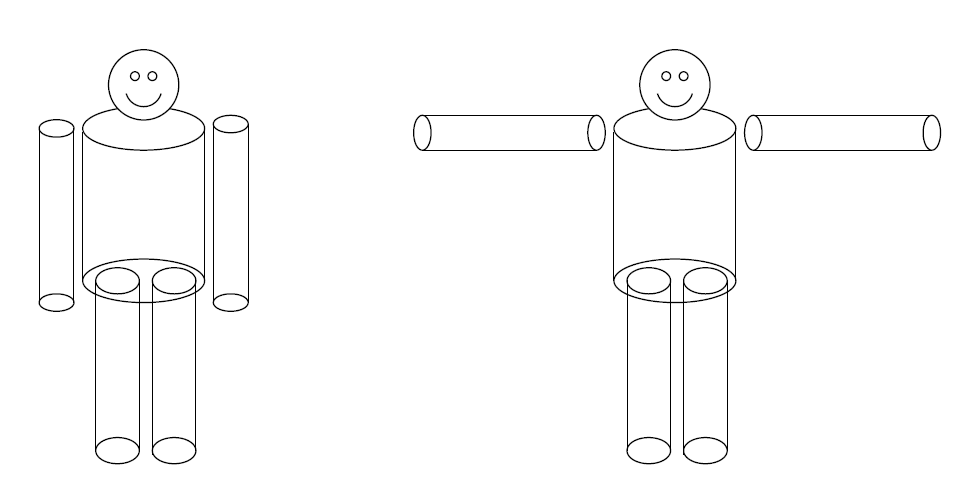
\includegraphics[scale=.4]{content/images/Puppe.png} 
\caption{Die Haltungen der Puppe mit angelegten und mit ausgestreckten Armen.\cite{V101}}
\label{fig:Puppe}
\end{figure}

\subsubsection{Puppe mit ausgebreiteten Armen und geschlossenen Beinen}

\noindent Für den Mittelwert von $T$ ergibt sich mit den Werten für die Periodendauer $T$ aus Tabelle \ref{tab:tab6} mit Formel \eqref{eq:Tq} und \eqref{eq:sT}:
\[\bar{T}=\SI{1.27(1)}{\second}\] 
Aus Formel \eqref{eq:I_K} folgt für das Trägheitsmoment der Puppe mit ausgebreiteten Armen:
\[I_.{Puppe,ausg}=\SI{-2,2(1)e-3}{\kilo\gram\metre\squared}\]
Der Fehler errechnet sich dabei mit Formel \eqref{eq:sIK}.
Der genäherte Theoriewert berechnet sich mit den Werten aus Tabelle \ref{tab:tab5} durch die Summe der Trägheitsmomente der einzelnen Körper (vgl. Gleichung \eqref{eq:I_S}) und mit dem Satz von Steiner \eqref{eq:Satz von Steiner}:
\begin{align*}
I_.{Puppe,aus,theo} &= I_.{Rumpf}+I_.{Kopf}+2\left(I_.{Bein}+m_.{Bein}\left(\frac{d_.{Bein}}{2}\right)^2\right)\\
					&+2\left(I_.{Arm,HZ}+m_.{Arm}\left(\frac{d_.{Rumpf}+h_.{Arm}}{2}\right)^2\right)\\
					&\approx\SI{1,05e-3}{\kilo\gram\metre\squared}\text{.}
\end{align*}
Dabei berechnen sich $I_.{Rumpf}$ und $I_.{Bein}$ nach Formel \eqref{eq:I_SZ}. $I_.{Arm,HZ}$ berechnet sich nach Formel \eqref{eq:I_SZH} und $I_.{Kopf}$ berechnet sich nach Formel \eqref{eq:I_SK}.
\begin{table}
	\centering
	\caption{Messdaten zur Periodendauer einer Puppe mit ausgebreiteten Armen, wobei $T_.{mess}$ das vierfache der Periodendauer darstellt.}
	\sisetup{table-format=1.2}
	\begin{tabular}{S[table-format=1.2]S[table-format=1.2]}
		\toprule
		{$T_.{mess}/\si[per-mode=reciprocal]{\second}$} &{$T/\si[per-mode=reciprocal]{\second}$} \\
		\midrule
		5,09 & 1,27 \\
		5,12 & 1,28 \\
		5,00 & 1,25 \\
		5,07 & 1,27 \\
		5,03 & 1,26 \\
		\bottomrule
	\end{tabular}
	\label{tab:tab6}
\end{table}

\subsubsection{Puppe mit angelegten Armen und geschlossenen Beinen}

\noindent Für den Mittelwert von $T$ ergibt sich mit den Werten für die Periodendauer $T$ aus Tabelle \ref{tab:tab7} mit Formel \eqref{eq:Tq} und \eqref{eq:sT}:
\[\bar{T}=\SI{0.89(0)}{\second}\] 
Aus Formel \eqref{eq:I_K} ergibt sich für das Trägheitsmoment der Puppe mit angelegten Armen:
\[I_.{Puppe,ang}=\SI{-2,71(1)e-3}{\kilo\gram\metre\squared}\]
Der Fehler errechnet sich dabei mit Formel \eqref{eq:sIK}.
Der genäherte Theoriewert berechnet sich mit den Werten aus Tabelle \ref{tab:tab5} durch die Summe der Trägheitsmomente der einzelnen Körper (vgl. Gleichung \eqref{eq:I_S}) und mit dem Satz von Steiner \eqref{eq:Satz von Steiner}:
\begin{align*}
I_.{Puppe,an,theo} &= I_.{Rumpf}+I_.{Kopf}+2\left(I_.{Bein}+m_.{Bein}\left(\frac{d_.{Bein}}{2}\right)^2\right)\\
					&+2\left(I_.{Arm}+m_.{Arm}\left(\frac{d_.{Rumpf}+d_.{Arm}}{2}\right)^2\right)\\
					&\approx \SI{1,11e-4}{\kilo\gram\metre\squared} \text{.}
\end{align*}
Dabei berechnen sich $I_.{Rumpf}$, $I_.{Arm}$ und $I_.{Bein}$ nach Formel \eqref{eq:I_SZ}. $I_.{Kopf}$ berechnet sich nach Formel \eqref{eq:I_SK}.
\begin{table}
	\centering
	\caption{Messdaten zur Periodendauer einer Puppe mit angelegten Armen, wobei $T_.{mess}$ das vierfache der Periodendauer darstellt.}
	\sisetup{table-format=1.2}
	\begin{tabular}{S[table-format=1.2]S[table-format=1.2]}
		\toprule
		{$T_.{mess}/\si[per-mode=reciprocal]{\second}$} &{$T/\si[per-mode=reciprocal]{\second}$} \\
		\midrule
		3.55 & 0,89 \\
		3.58 & 0,90 \\
		3.56 & 0,89 \\
		3.55 & 0,89 \\
		3.53 & 0,88 \\
		\bottomrule
	\end{tabular}
	\label{tab:tab7}
\end{table}